%%%%%%%%%%%%%%%%%%%%%%%%%%%%%%%%%%%%%%%%%%%%%%%
%
% Template per Elaborato di Laurea
% DISI - Dipartimento di Ingegneria e Scienza dell’Informazione
%
% update 2015-09-10
%
% Per la generazione corretta del 
% pdflatex nome_file.tex
% bibtex nome_file.aux
% pdflatex nome_file.tex
% pdflatex nome_file.tex
%
%%%%%%%%%%%%%%%%%%%%%%%%%%%%%%%%%%%%%%%%%%%%%%%

% formato FRONTE RETRO
\documentclass[epsfig,a4paper,11pt,titlepage,twoside,openany]{book}
\usepackage{epsfig}
\usepackage{plain}
\usepackage{setspace}
\usepackage[paperheight=29.7cm,paperwidth=21cm,outer=1.5cm,inner=2.5cm,top=2cm,bottom=2cm]{geometry} % per definizione layout
\usepackage{titlesec} % per formato custom dei titoli dei capitoli

%%%%%%%%%%%%%%
% supporto lettere accentate
%
%\usepackage[latin1]{inputenc} % per Windows;
\usepackage[utf8x]{inputenc} % per Linux (richiede il pacchetto unicode);
%\usepackage[applemac]{inputenc} % per Mac.

\singlespacing

\usepackage[english]{babel}

\usepackage{float} % posizionamento immagini

% tabelle
\usepackage{booktabs}
\usepackage{tabularx}

\begin{document}

  % nessuna numerazione
  \pagenumbering{gobble} 
  \pagestyle{plain}

\thispagestyle{empty}

\begin{center}
  \begin{figure}[h!]
    \centerline{
\psfig{file=figures/logo_unitn_black_center.eps,width=0.6\textwidth}}
  \end{figure}

  \vspace{2 cm} 

  \LARGE{Department of Information Engineering and Computer Science\\}

  \vspace{1 cm} 
  \Large{Bachelor's Degree in\\
    Computer Science
  }

  \vspace{2 cm} 
  \Large\textsc{Final Dissertation\\} 
  \vspace{1 cm} 
  \Huge\textsc{A blockchain-based solution for logistics tracking\\}


  \vspace{2 cm} 
  \begin{tabular*}{\textwidth}{ c @{\extracolsep{\fill}} c }
  \Large{Supervisor} & \Large{Student}\\
  \Large{prof. Montresor Alberto}& \Large{Melotti Damiano}\\
  \end{tabular*}

  \vspace{2 cm} 

  \Large{Academic year 2018/2019}
  
\end{center}



  \clearpage
 
%%%%%%%%%%%%%%%%%%%%%%%%%%%%%%%%%%%%%%%%%%%%%%%%%%%%%%%%%%%%%%%%%%%%%%%%%%
%%%%%%%%%%%%%%%%%%%%%%%%%%%%%%%%%%%%%%%%%%%%%%%%%%%%%%%%%%%%%%%%%%%%%%%%%%
%% Nota
%%%%%%%%%%%%%%%%%%%%%%%%%%%%%%%%%%%%%%%%%%%%%%%%%%%%%%%%%%%%%%%%%%%%%%%%%%
%% Sezione Ringraziamenti opzionale
%%%%%%%%%%%%%%%%%%%%%%%%%%%%%%%%%%%%%%%%%%%%%%%%%%%%%%%%%%%%%%%%%%%%%%%%%%
%%%%%%%%%%%%%%%%%%%%%%%%%%%%%%%%%%%%%%%%%%%%%%%%%%%%%%%%%%%%%%%%%%%%%%%%%%
  \thispagestyle{empty}

\begin{center}
  {\bf \Huge Acknowledgments}
\end{center}

\vspace{4cm}


\emph{
%  The first thanks goes to Prof. Montresor, for his guidance and constant support during the work of this thesis. His knowledge and patience have been fundamental to achieve a good result. I would also like to thank the Spindox Labs team, for giving me the opportunity of studying and exploring these technologies. I am specially thankful to Filippo, who has been not only a roommate, but also a valuable friend and an endless source of inspiration and advice. His presence accompanied me during my bachelor studies and he totally deserves my gratitude. Last, but not least, a sincere thanks to my family and my girlfriend, for being always by my side and supporting me in every moment of these years.
The first thanks goes to Prof. Montresor, for his guidance and constant support during the work of this thesis. His knowledge and patience have been fundamental to achieve a good result. I would also like to thank the Spindox Labs team, for giving me the opportunity of studying and exploring these technologies. I am thankful to my family and my girlfriend, for being always by my side and supporting me in every moment of these years. Finally, a special thanks to Filippo, who has been not only a roommate, but also a valuable friend and an endless source of inspiration and advice. His presence accompanied me during my bachelor studies and he totally deserves my gratitude.
}

  \clearpage
  \pagestyle{plain} % nessuna intestazione e pie pagina con numero al centro

  
  % inizio numerazione pagine in numeri arabi
  \mainmatter

%%%%%%%%%%%%%%%%%%%%%%%%%%%%%%%%%%%%%%%%%%%%%%%%%%%%%%%%%%%%%%%%%%%%%%%%%%
%%%%%%%%%%%%%%%%%%%%%%%%%%%%%%%%%%%%%%%%%%%%%%%%%%%%%%%%%%%%%%%%%%%%%%%%%%
%% Nota
%%%%%%%%%%%%%%%%%%%%%%%%%%%%%%%%%%%%%%%%%%%%%%%%%%%%%%%%%%%%%%%%%%%%%%%%%%
%% Si ricorda che il numero massimo di facciate e' 30.
%% Nel conteggio delle facciate sono incluse 
%%   indice
%%   sommario
%%   capitoli
%% Dal conteggio delle facciate sono escluse
%%   frontespizio
%%   ringraziamenti
%%   allegati    
%%%%%%%%%%%%%%%%%%%%%%%%%%%%%%%%%%%%%%%%%%%%%%%%%%%%%%%%%%%%%%%%%%%%%%%%%%
%%%%%%%%%%%%%%%%%%%%%%%%%%%%%%%%%%%%%%%%%%%%%%%%%%%%%%%%%%%%%%%%%%%%%%%%%%

    % indice
    \tableofcontents
    \clearpage
    
    
          
    % gruppo per definizone di successione capitoli senza interruzione di pagina
    \begingroup
      % nessuna interruzione di pagina tra capitoli
      % ridefinizione dei comandi di clear page
      \renewcommand{\cleardoublepage}{} 
      \renewcommand{\clearpage}{} 
      % redefinizione del formato del titolo del capitolo
      % da formato
      %   Capitolo X
      %   Titolo capitolo
      % a formato
      %   X   Titolo capitolo
      
      \titleformat{\chapter}
        {\normalfont\Huge\bfseries}{\thechapter}{1em}{}
        
      \titlespacing*{\chapter}{0pt}{0.59in}{0.02in}
      \titlespacing*{\section}{0pt}{0.20in}{0.02in}
      \titlespacing*{\subsection}{0pt}{0.10in}{0.02in}
      
      % sommario
      \chapter*{Abstract} % senza numerazione
\label{abstract}

\addcontentsline{toc}{chapter}{Abstract} % da aggiungere comunque all'indice

%\textit{Hints provided by the template:}
\iffalse



  Sommario è un breve riassunto del lavoro svolto dove si descrive l'obiettivo, l'oggetto della tesi, le 
metodologie e le tecniche usate, i dati elaborati e la spiegazione delle conclusioni alle quali siete arrivati.  

Il sommario dell’elaborato consiste al massimo di 3 pagine e deve contenere le seguenti informazioni:
\begin{itemize}
  \item contesto e motivazioni 
  \item breve riassunto del problema affrontato
  \item tecniche utilizzate e/o sviluppate
  \item risultati raggiunti, sottolineando il contributo personale del laureando/a
\end{itemize}

\fi

All logistic processes involve the exchange of goods between entities that do not fully trust each other. For example, let us consider a very common scenario: a delivery by a courier that includes an intermediate stop. This can be the porter of a building, or an authorized post office. What usually happens is that when the parcel arrives, the receiver testifies with his/her signature (on paper or on an electronic device) that the exchange has occurred. However, this is not always true, because not all the deliveries include this possibility or because the persons directly performing the exchange do not fully respect the protocol. As a result, the process is vulnerable: a hand-written signature is often counterfeitable and when it is not even present, it is possible to generate a debate ``my word against yours''.

This problem becomes worse when it includes more steps: this happens, for example, in complex systems of organizations, people and activities employed in the supply chain sector: here the handovers are even more articulated and it is important to guarantee a successful outcome of the processes, that are crucial for the companies involved. A series of signatures can be a solution, but, as aforementioned, several things can go wrong.

Who has not been taken into consideration yet is the final recipient. They know nothing about the events happening and they could only be notified autonomously by one of the entities involved, whom they would have to trust. 

Together with the \textsc{Spindox Labs} team, we tried to investigate a solution to this problem. We started from the wide experience that the company had with trackers, trying to understand if one of them could be applicable to this case. IoT devices are spreading more and more thanks to the many applications they have. Both industry and research are very active in this area, hence we had to conduct an in-depth analysis to explore the various alternatives available. We eventually found a good solution, that meets our requirements for communication, connectivity and geolocation. After this, the most significant part of our research involved the study on the architecture that our system required. We wanted to find an innovative solution that eliminated any centralized authority, because did not want to introduce one in the system: many entities at the same level, without a supervising one. 

The result of this work is a decentralized architecture approaching the problem with a combination of diverse technologies. We implemented a private blockchain, to guarantee distribution and reliability, we integrated IoT devices to track the deliveries and we included web servers and interfaces to facilitate the usage of the service. This project has been a research activity, thus no specific requirements from any client have been considered. The solution is a ``proof-of-concept'', demonstrating the power of the technologies involved and it can represent a complete starting base for a customized version, tackling a particular problem.

The dissertation is organized as follows: Chapter~\ref{cha:scenario} and~\ref{cha:main} introduce the problem and present the architecture. Then the proposed solution is split into its three main components, namely tracking, decentralization and servers. Chapter~\ref{cha:future} evaluates the project, outlining limits and possible extensions. Chapter~\ref{cha:conclusion} concludes the thesis.

\newpage
%%%%%%%%%%%%%%%%%%%%%%%%%%%%%%%%%%%%%%%%%%%%%%%%%%%%%%%%%%%%%%%%%%%%%%%%%%
%%%%%%%%%%%%%%%%%%%%%%%%%%%%%%%%%%%%%%%%%%%%%%%%%%%%%%%%%%%%%%%%%%%%%%%%%%
%% Nota
%%%%%%%%%%%%%%%%%%%%%%%%%%%%%%%%%%%%%%%%%%%%%%%%%%%%%%%%%%%%%%%%%%%%%%%%%%
%% Sommario e' un breve riassunto del lavoro svolto dove si descrive 
%% l’obiettivo, l’oggetto della tesi, le metodologie e 
%% le tecniche usate, i dati elaborati e la spiegazione delle conclusioni 
%% alle quali siete arrivati.
%% Il sommario dell’elaborato consiste al massimo di 3 pagine e deve contenere le seguenti informazioni: 
%%   contesto e motivazioni
%%   breve riassunto del problema affrontato
%%   tecniche utilizzate e/o sviluppate
%%   risultati raggiunti, sottolineando il contributo personale del laureando/a
%%%%%%%%%%%%%%%%%%%%%%%%%%%%%%%%%%%%%%%%%%%%%%%%%%%%%%%%%%%%%%%%%%%%%%%%%%
%%%%%%%%%%%%%%%%%%%%%%%%%%%%%%%%%%%%%%%%%%%%%%%%%%%%%%%%%%%%%%%%%%%%%%%%%%      
      
      %%%%%%%%%%%%%%%%%%%%%%%%%%%%%%%%
      % lista dei capitoli
      %
      % \input oppure \include
      %
      \chapter{The scenario}
\label{cha:scenario}
%\textit{Detailed explanation of the problem and its scope: starting from a practical description, a formalization of the entities involved and what they want to achieve. 2 examples (deliveries with couriers and port exchanges). Then, the intentions of the company I have worked for.}

This chapter introduces the problem, giving a more detailed description. In fact, we have only given a few examples in the Summary, but we need a precise model of the use case. Then we focus on decentralization, explaining what the main characteristics of such approach are and defining some concepts.

\section{Problem statement and solution architecture}
\label{sec:statement}
Formalizing the problem, the typical scenario is the following. We have a sender \textit{S} and a final recipient \textit{R}. \textit{S} wants to send \textit{R} a particular good, \textit{G}. To perform the exchange, \textit{S} will designate a certain route that involves \textit{n} intermediate stops ($I_1, I_2, ..., I_n$) and will instruct \textit{m} dealers ($D_1, D_2, ..., D_m$) that will take care of each part of the delivery. From a theoretical point of view, nothing forbids to have two identical dealers $D_i$ - $D_j$. Indeed, as we will see later, we are not really interested in the dealers themselves, but more in the companies that these dealers work for. We assume that \textit{S} decides the route or, at least, knows the various stops needed.

We would like to find a model able to register precisely each handover, by making use of secure techniques that do not allow counterfeiting or fraud: each entity should be protected against a potential malicious one. Finally, \textit{R} should be able to monitor the events about \textit{G}, in order to check the progresses.

The proposed solution will make use of IoT devices to track the location of the dealers. Additionally, we will define a protocol to use the connectivity of these trackers to detect other devices owned by the intermediate points. In this way, the verification will be automatized and, from the human point of view, we will only need a little expedient from the dealers. Furthermore, the architecture will not present any centralized element: the solution will be fully decentralized.

\section{Decentralization}
\label{sec:decentralization}
%\textit{Why decentralization can be the solution, how it differs from a traditional approach. The blockchain, with its hype, as a valid alternative. Deep explanation of what it is etc.}

Unlike traditional architectures, that usually present a single element providing all the information for the service and practically having control, a typical distributed network shares knowledge between many nodes, therefore excluding a central point.

Centralization versus decentralization is a battle that does not have a definite winner. The Internet has seen several attempts to decentralize some services, like DNS and social networks, but the truth is that, in many situations, the benefits of keeping a central entity often outperform those of the correspondent distributed alternatives~\cite{Montresor_Permissionless}. However, there are still some cases in which a P2P network is a valid solution, especially when there are hard requirements like privacy, anti-censorship and scalability. Despite their advantages, in fact, centralized architectures always present a single point of failure, with all its consequences.

When in 2008 the mysterious Satoshi Nakamoto published the Bitcoin paper~\cite{bitcoin}, a particular type of distributed network became extremely popular: the \emph{blockchain}. The author proposed ``a purely peer-to-peer version of electronic cash'', with the aim of introducing a payment system based on a crypto-currency, without intermediaries but still reliable and secure against typical attacks such as double spending. This problem may arise for two reasons. The first is that crypto-currencies have no watermarks to prevent the unauthorized production of money: consequently, it is in principle possible to copy one coin and spend it twice. The second is a direct disadvantage of a distributed system: propagation delays have to be handled in order, to successfully distinct and validate the correct transactions. More generally, distributed networks need to implement a protocol to establish consensus between nodes.
Bitcoin combines existing technologies in a sophisticated way, to solve its fundamental problems. Without examining in depth all these mechanisms, let us concentrate on how transactions are stored: using a blockchain.

The blockchain itself is just a distributed data structure: as the name suggests, it is composed by blocks and each block contains transactions. These transactions are defined with a precise grammar, that obviously depends on the type of application. In Bitcoin, for example, transactions respect the (simplified) form ``the result of transaction $T_i$ is used as input to send $x$ BTC to $A$, with fee $y$'', where $A$ is the public key of the recipient. Beyond the grammar, to implement a blockchain there is the need of a function to validate transactions. Evidently, the previous sample transaction will be refused, if the sender does not have the rights to use the output of $T_i$. More precisely, Bitcoin uses a measure called proof-of-work, in order to not only include a control on the actual validity of the transactions, but also to require a strong computational effort to approve a block. This is a crucial element to improve reliability and contrast the possibility of subverting the network with Sybil attacks.

What makes the blockchain different from other data structures are two properties. First, it is distributed: every node of the network has its own copy of a \emph{ledger}, that is kept consistent and up to date with gossip protocols. Second, the way in which these blocks are linked: each one contains the hash fingerprint of the previous. As a result of these, once data is inserted in a block it impossible to change it. In practice, changing a transaction would mean recalculating the hash value of all the blocks succeeding the modified one, replacing the fingerprint and convincing all the network that the new copy is the one that should be used. This is impossible, unless one controls more than half of the overall computing power. Immutability is the first and fundamental property of the blockchain, that makes it a good solution to store money exchanges: obviously, crypto-currency designers do not want to allow the possibility of modifying any of the validated transactions.

The Bitcoin system showed the world the great potential of the blockchain. After its success, a number of other similar crypto-currencies were launched, with the so-called \emph{initial coin offerings}, generating a new business for investors and speculators. A lot of hype is still surrounding this technology, that in any case presents some disadvantages and it is surely not the right solution for every problem~\cite{noblockchain}. 

Analyzing again our case, however, it seems to suit well. Handovers can correspond to the transactions, the goods can be our ``coins'' and the entities of the system can be the participants of the network, submitting exchanges. Essential requirements such as reliability and durability of transactions would be guaranteed by design. In Chapter~\ref{sec:arch} we discuss better this approach.


      \chapter{The solution}
\label{cha:main}
%\textit{Schema of the final solution, explanation of the flow and how it concretely works. Then, focus on three key components.}

Figure \ref{fig:solution} illustrates the solution that we have designed. Let us explain its characteristics, by first analyzing the overall flow and then concentrating on each step.

The notation used in the schema is the same as the one introduced in Section \ref{sec:statement}: from left to right, we notice the sender \textit{S}, the good \textit{G}, two dealers $D_1$ and $D_2$, two intermediate points $I_1$ and $I_2$ (each one with a responsible person at work) and finally the receiver $R$. Obviously, this scenario is just a possible combination of entities and the solution is not fixed to this one.

The following is an abstract description of the various actions that are part of the model. For this moment we are ignoring some specific details (e.g. the protocols used for interactions, the format of the packets etc.), that will be properly explained together with the singular components.

$S$ starts the process by inserting into the system the information related to $G$. They have a dedicated server to provide the requested data. In particular, they need to declare the intermediate points and the dealers. This data will be stored in the blockchain as a new ``asset'', something similar to the coins in crypto-currencies. 

Then, the delivery is ready to start. $D_i$ (the procedure holds for both $D_1$ and $D_2$) carries an IoT device tracking its location and searching for other BLE devices nearby. On the other side, the intermediate stop has a beacon, constantly advertising its UUID (Universally Unique IDentifier). The protocol for the exchange is the following: 
\begin{itemize}
    \item The dealer arrives at the destination, the tracker detects the stop and sends to a server a packet containing the beacons' identifiers found;
    \item The server controls if one of the identifiers corresponds to the one owned by the intermediary and, if so, sends a confirmation to the blockchain;
    \item The person in control of $I_j$ collects $G$ and sends a confirmation, using a web interface, to a separate web server.
\end{itemize}

\begin{figure}[h]
    \centering
    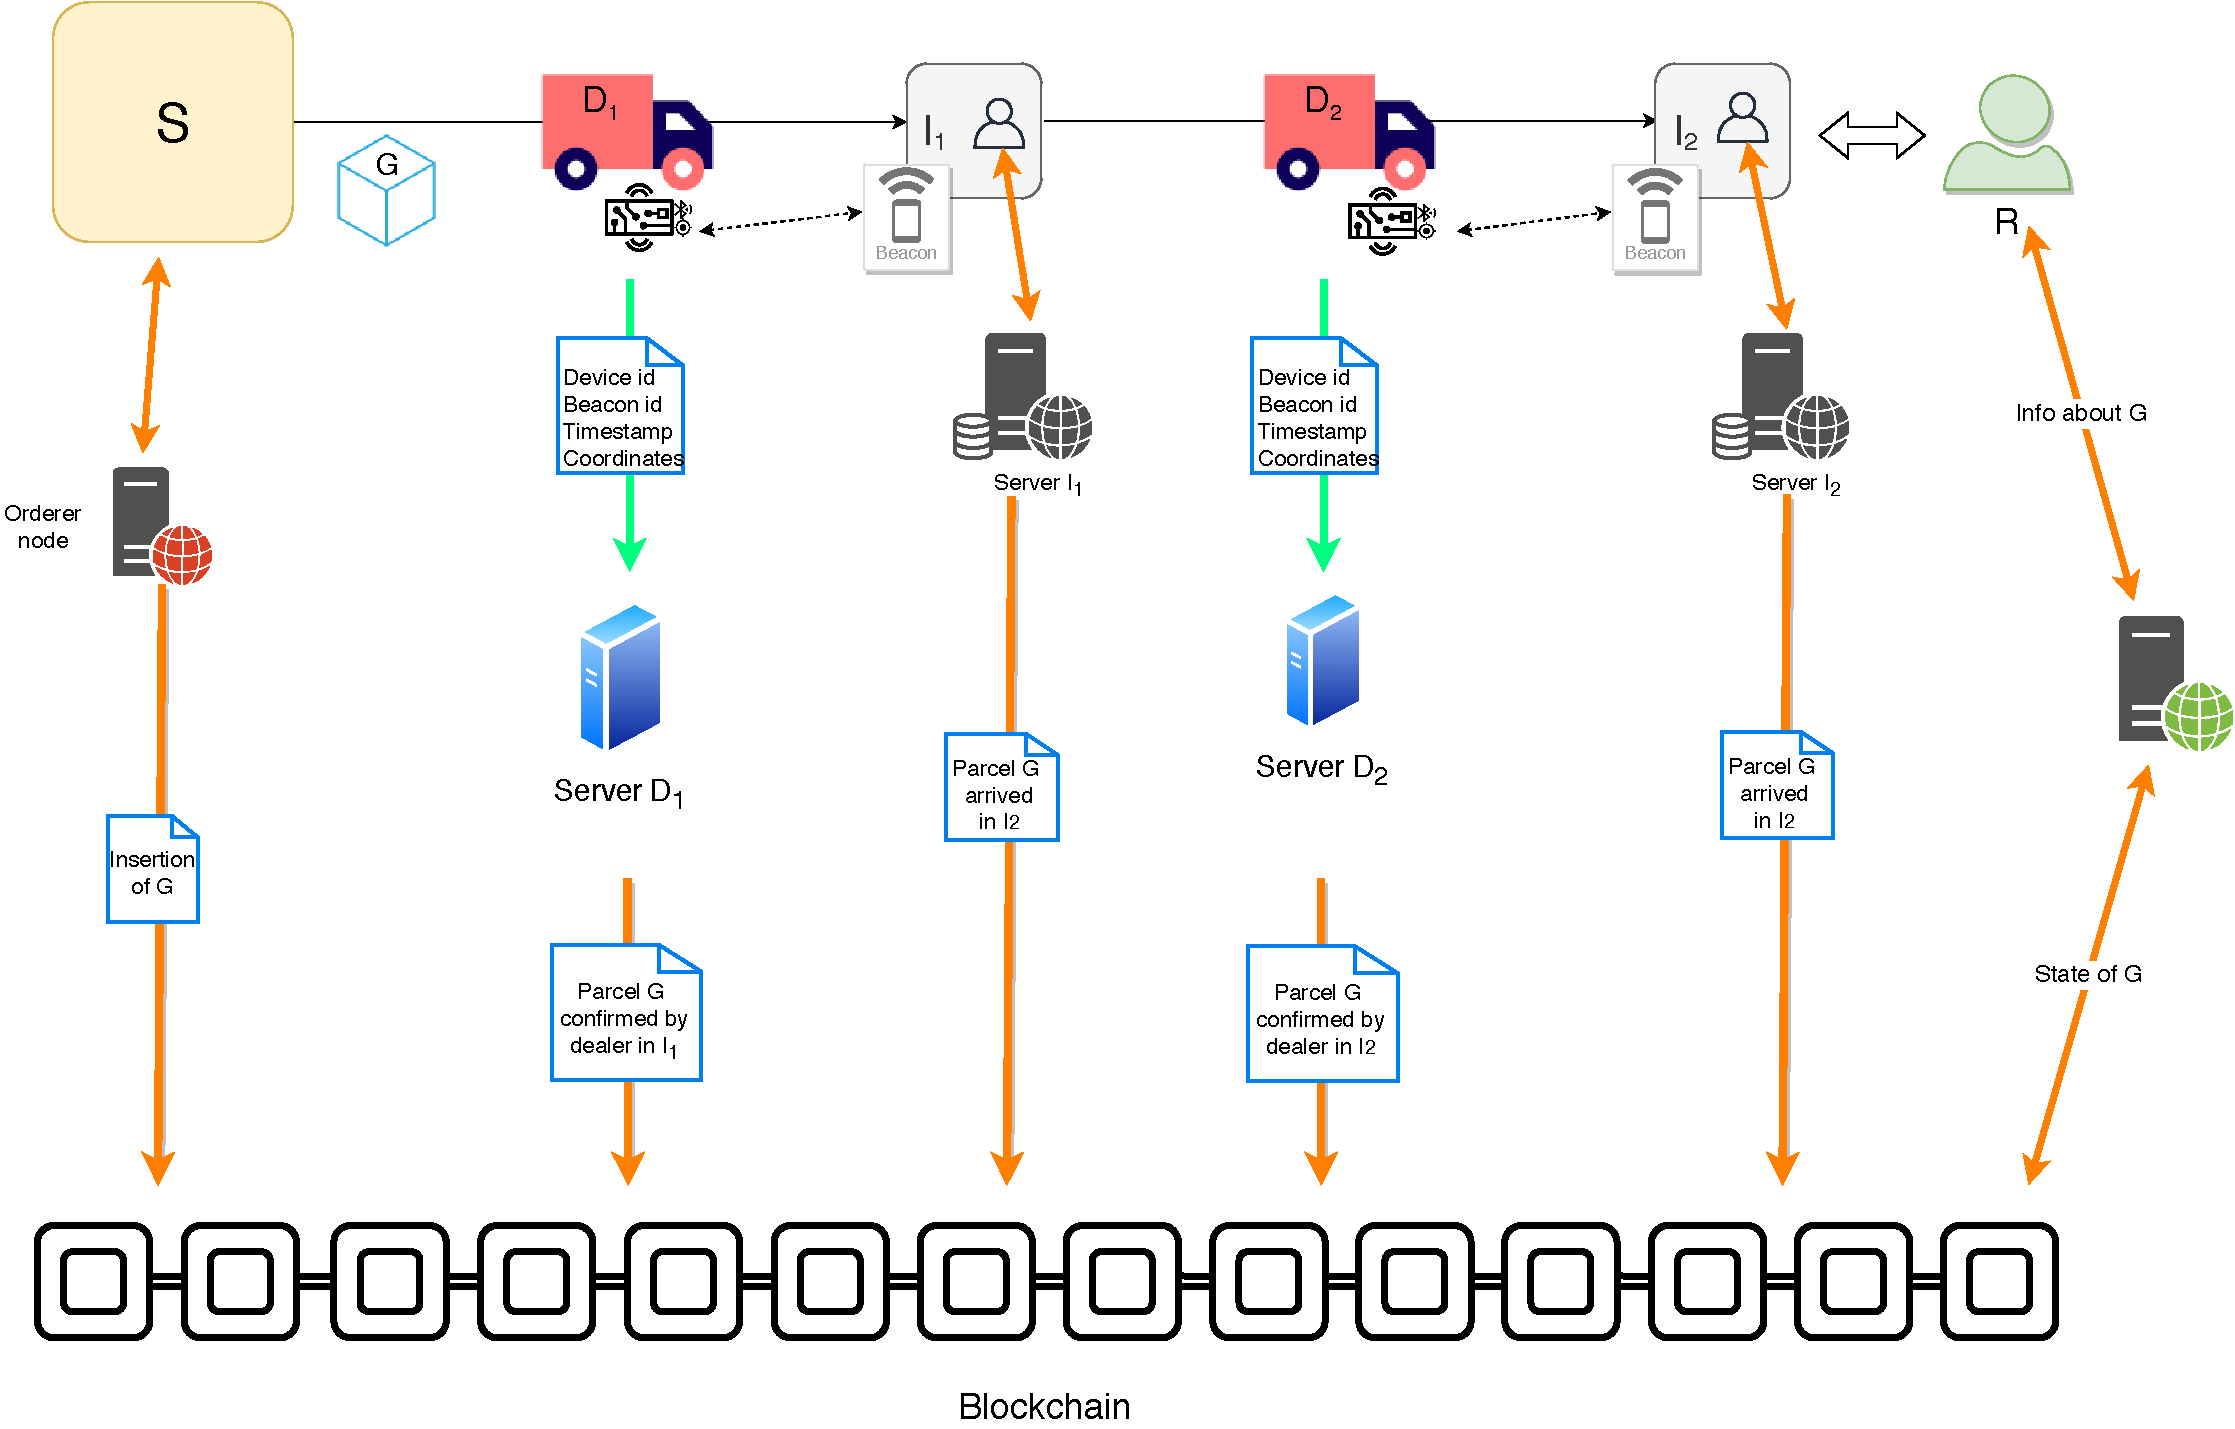
\includegraphics[width=\textwidth]{figures/solution.pdf}
    \caption{The schema of the discussed solution}
    \label{fig:solution}
\end{figure}

The model as it is so far cannot be deceived by the dealer, as they have no control over the device; however, it is vulnerable to an attack from a malicious actor controlling $I$. They can, in fact, collect $G$ and not inform the system about the exchange. As a result, we have lost track of who has the good. To solve this, there is the need for a protocol on the human side. Not complicated, but essential: the dealer has to make sure that who receives $G$ really sends their confirmation to the server. 

The final recipient, at any time, can access an interface that, by consulting the status of G on the blockchain, informs him about the progress of the delivery. They can check which exchanges happened and whether they succeeded. In case of problems it is immediate to find the responsible. Assuming that the protocol has been fully respected, if $G$ is only confirmed by the dealer, it means that it is still in their hands; to the contrary, if only the intermediary confirmed the good, an error must have occurred, because there is no proof that the dealer really arrived at that place.

After this brief analysis there are a lot of unknown elements: how the devices work, how the communications take place, how data is actually saved. In the next chapters we will discuss these aspects, dividing the project into the three main branches that constitute it.


\chapter{Tracking}
\label{sec:tracking}
%Introduction to what kind of tracking is needed, what we expect from the devices. Brief explanation of the state of the art of communication technologies (LoRa, SigFox, LTE, Wi-Fi, BLE, ...) and geolocation.

The first part that we analyze is the tracking. Our solution needs devices that support geolocation, bluetooth and can connect to the Internet to send messages. Clearly these are just the basic requirements, additional features can be useful in future developments. Another important aspect is the battery, since these devices cannot ensure long autonomy if frequently active. 

First, we will give a brief description of the modern technologies for the communications of IoT devices, then we will dive into the market to analyze the various options.

\section{Communication technologies}
\label{sec:track_comm}
%\textit{A brief analysis over the existing tracking technologies}

The state-of-the-art of these networks is very wide and presents several alternatives, each of them with advantages and disadvantages. They can be divided by many parameters, since many variables need to be taken into account when modelling the architecture of an IoT project. Our use case requires a standard able to guarantee the delivery of packets at arbitrary distance, consuming as little battery as possible. These requirements drive us to a new wireless communication techonology: LPWAN (Low Power Wide Area Network).

LPWAN is increasingly becoming popular thanks to its low-power, long-range and low-cost communication properties. It is particularly suitable for IoT applications that only need to transmit small amounts of data in long range and for its specifications it is preferable to traditional cellular options (such as 4G and LTE networks).

Many LPWAN technologies have been developed in both the licensed and unlicensed frequency bands. LoRa, Sigfox and NB-IoT are today the leading ones, with many technical differences \cite{LPWAN_study}.

\subsubsection{LoRa}
LoRa (Long Range) is a patented digital wireless communication technology that was first developed by Cycleo - a French start-up - and then acquired by Semtech (USA). Its ecosystem can be divided in two parts, LoRa and LoRaWAN: the latter is the standard protocol for WAN communications and the former is used as a wide area network technology. In other words, LoRa is the physical layer and LoRaWAN is the MAC and application layer of the stack.

LoRaWAN provides various classes of end devices to satisfy different requirements. It ensures a better battery life compared to the other LPWAN technologies, but this also implies lower data rates and longer latency. To connect to the Internet, LoRa requires a gateway. The infrastructure is the following: end devices communicate with one or more LoRa gateways, which then forward messages to a cloud, a network server or to another gateway. On the contrary, when a message is sent to a device, the network chooses the best gateway.

One important aspect of LoRaWAN is determined by the so-called duty-cycle: defined as the maximum percentage of time during which an end-device can occupy a channel, is a key constraint for networks operating in unlicensed bands. Thus, each device has a threshold limiting the overall transmission time. However, the amount of time that a device will need is unknown, since it depends on the distance between the end point and the nearest gateway. The farther the gateway, the longer it will take to deliver a message. As a result, the total amount of messages sent is unknown and totally unpredictable considering our use case, in which we cannot make assumptions on the distribution of the gateways (w.r.t. the location of the tracker).

%To sum up: LoRaWAN is not proprietary and offers quite a good amount of flexibility, but it has some problems of coverage and infrastructure that does not make it the best choice.

\subsubsection{Sigfox}
Sigfox is a patented technology that was developed in 2010 by the start-up SigFox. It is an LPWAN network operator that uses a wide-reaching signal called ``ultra narrow-band''. This system presents a significant link asymmetry: a downlink communication, i.e., data from the base stations to the end devices can only occur following an uplink communication and in every case the number of messages is limited to 4 per day. On the uplink, instead, the amount of packets sent cannot be more than 140 per day, with a maximum payload length of 12 bytes. These limitations are similar to the LoRa's ones: in fact, they were included by the designers for the same reasons. Clearly, acknowledgements cannot be supported and consequently the reliability is ensured using time and frequency diversity as well as transmission duplication.

\subsubsection{NB-IoT}
NB-IoT is a radio technology standard developed by 3GPP (3rd Generation Partnership Project) to enable a wide range of cellular devices and services. It is based on the LTE protocol, therefore guaranteeing the high performance level associated with cellular connections, but at the cost of more complexity and greater power consumption. While other infrastructures have gateways that aggregate sensor data, which then communicate with the primary server, with NB-IoT sensor data is sent directly to it. For this reason it is being touted as the potentially less expensive option.

LTE-M is another LPWAN radio technology standard based on LTE. However, we did not take it into consideration because there is a lack of coverage and support from operators in Italy.

%We can conclude that, for our use case, the NB-IoT is the best alternative: despite the higher battery usage, it offers a solid and unrestricted network that can be used without creating a particular infrastructure or having to limit the number of messages.


\section{The market}
\label{sec:market}
%\textit{The study and testing of the alternatives available, maybe a table summarizing the characteristics of each device (type of communication supported, battery, personalization of firmware, cost).}

The market of the IoT is constantly growing. There are numerous applications for these devices, both indoors and outdoors, with a variety of different requirements. For this reason, almost every company offers more than one solution, to best meet the needs of the buyer. We proceed now with the analysis of some candidate trackers. Table \ref{table_devices} summarizes their technical features.

\begin{table}[htbp]
\centering
\newcolumntype{Y}{>{\raggedright \arraybackslash}X}
\begin{tabularx}{\textwidth}{YYYYYY}
\toprule
\textbf{Company}        & \textbf{Device}         & \textbf{Connectivity}                                                          & \textbf{GNSS}                                & \textbf{Customizable firmware}           & \textbf{Additional}                                           \\ \midrule
Estimote       & LTE beacon     & Bluetooth 5.0, LTE-M/NB-IoT, NFC                                      & GPS, GALILEO, GLONASS               & No, but scripts can be included & accelerometer, temperature, LED, programmable button \\ \midrule
Accent Systems & IoT tracker    & Bluetooth 5.0, Wi-Fi, LTE-M/NB-IoT                                    & GPS, GLONASS, Galileo, QZSS, BeiDou & No                              & accelerometer, temperature, LED, buzzer              \\ \midrule
Sensolus       & Ultra          & BLE, Wi-Fi, Sigfox, GPS                                               & GPS                                 & No, but cloud API available     & accelerometer, temperature                           \\ \midrule
Pycom          & FiPy + PyTrack & Bluetooth, Wi-Fi, LTE-M/NB-IoT, LoRa, Sigfox & GPS, GLONASS, Galileo, QZSS         & Yes                             & accelerometer, LED                                   \\ \bottomrule
\end{tabularx}
\caption{Specifications of the devices}
\label{table_devices}
\end{table}

\subsubsection{Estimote, LTE beacon}
Estimote, Inc. \cite{estimote} is an American company that offers mostly beacons of different types. Their main focus is in indoor applications, but they also offer a device particularly close to our needs: the LTE beacon.

This tracker can connect to the Estimote cloud over LTE. Through this platform it is possible to include JavaScript code that will be run by the device, but the firmware itself is not customizable. This is the first negative point: every communication of the device is directed to its cloud and it is not possible to bypass it. Furthermore, the LTE beacon comes with a subscription including 1000 syncs per year per each device (for example, about 2-3 syncs per day). There’s also a data-cap of 100 MB per year.

%Even though the tracker offers a very good range of sensors and built-in radios, the limitations on the number of packets and the necessity to pass from its cloud make us definitely discard this candidate.
The tracker offers a good range of sensors and built-in radios. On the other hand, though, Estimote claims that, if frequently synced with the server, the battery life will be shorter than 2 days. Consequently, choosing the LTE beacon would imply the need of an external power bank or a permanent connection to the vehicle.

\subsubsection{Accent Systems, IoT tracker}
Accent Systems \cite{accentsys} designs and develops tailored IoT devices, offering an end-to-end solution. Like Estimote, they have a wide range of beacons and one particular device for outdoor tracking via LPWANs, called IoT tracker.

This solution is not personalizable in any way. The firmware is not modifiable and it communicates with a platform called Inmolecular (over LTE), a built-in ecosystem to show the tracker's data. The device, as specified in the website, is more destined to be integrated in an asset or in a vehicle to track only its location, not really to send custom packets as our project requires. Nevertheless, its characteristics make it a valid alternative.

\subsubsection{Sensolus, Ultra}
Sensolus \cite{sensolus} is an industrial IoT company, based in Belgium. Their main offer is addressed to logistic companies that want to track their assets. Indeed they propose an easy and ready-to-go service, similarly to the Accent Systems' one. Ultra is the tracker that we considered as a potential solution.

This is another device not open to personalization. However, the cloud exposes numerous APIs to read data sent by the trackers: the overhead is still present, but our server could coexist. Concerning the battery, the presence of a replaceable one is a double-edged sword, because on the one hand it is can ensure longer life, but on the other it requires an action to change it.

This device only supports Sigfox connectivity: the APIs are actually an extension of those provided by the operator. As pointed out in the previous section, this communication technology has some limitations in the number of messages that can be sent, which inevitably affect this tracker too.

\subsubsection{Pycom, Fipy and PyTrack}
Pycom \cite{pycom} offers hardware products that vary from plug and play devices to single components such as development boards and accessories. There are two separate products that together can form a good tracking solution: a development board (FiPy) and an additional module to support geolocation (PyTrack).

This alternative is completely different from the other ones: instead of offering an entire environment, almost ready to use, this device comes completely empty and needs to be programmed. Even the battery is not present, so one can decide which one to use, or directly power it via cable. 

\section{The choice}
\label{sec:track_choice}
%\textit{Why we decided to choose that device: possibility to fully program the firmware, connectivity...}

Analyzing the various alternatives outlined we opted for the Pycom device. The first reason is the possibility of fully programming the firmware, which guarantees a high level of flexibility. Indeed, we need a complete control on the device: the algorithm needs to be elaborated and written by us. With all the other solutions, this would not possible; building our service on top of another one was not ideal.

In addition, the FiPy board offers a wide range of communication technologies that we could use: from the simple Wi-Fi for the developing phase to all the mentioned LPWANs. As for the latter, we identified NB-IoT as the best technology. Similarly to the previous decision, we made this choice because, despite the higher battery consumption, it offers a solid, reliable and unrestricted network, which can be used without creating a particular infrastructure or having to limit the number of messages.

\section{Firmware}
\label{sec:track_firmware}
%\textit{Life cycle of the device (maybe with a flow chart). Some snippets?}

% block styles
\tikzstyle{decision} = [diamond, draw, 
    text width=5.4em, text badly centered, node distance=3cm, inner sep=0pt]
\tikzstyle{block} = [rectangle, draw,
    text width=5em, text centered, minimum height=4em]
\tikzstyle{line} = [draw, -latex']
\tikzstyle{cloud} = [draw, ellipse,fill=red!20, node distance=3cm,
    minimum height=2em]
    
\begin{figure}[htb]
\begin{tikzpicture}[node distance = 3cm, auto]
	% nodes
	\node [cloud] (start) {Start};
	\node [block, right of=start, yshift=-3em] (lte) {Attach to LTE};
	\node [block, right of=lte, xshift=1em] (initble) {Init Bluetooth};
	\node [block, right of=initble, xshift=1em] (initgnss) {Init GNSS};
	\node [block, below of=initble, yshift=-1em] (coord) {Search coordinates};
	\node [decision, right of=coord, xshift=1em] (foundcoord) {Coordinates found?};
	\node [block, below of=foundcoord, xshift=6em, yshift=-1em] (ble) {BLE scan};
	\node [decision, below of=ble] (conn) {Connected?};
	\node [block, left of=conn, xshift=-1em] (save) {Save to file};
	\node [block, right of=conn, xshift=1em] (send) {Send data};
	\node [block, below of=conn] (sleep) {Sleep for X minutes};
	% edges
	\path [line] (start) |- (lte);
	\path [line] (lte) -- (initble);
	\path [line] (initble) -- (initgnss);
	\path [line] (initgnss.south) -| ++(0pt, -15pt) -| (coord.north);
	\path [line] (coord) -- (foundcoord);
	\path [line] (foundcoord.south) |- node [near start] {no} ++(0pt,-20pt) -| (coord);
	\path [line] (foundcoord.east) -| node [near start] {yes} ++(20pt,0pt) -| (ble);
	\path [line] (ble) -- (conn);
	\path [line] (conn) -- node [near start] {yes} (send);
	\path [line] (conn) -- node [near start] {no} (save);
	\path [line] (save.south) |- ++(0pt, -20pt) |- (sleep);
	\path [line] (send.south) |- ++(0pt, -20pt) |- (sleep);
	\path [line] (sleep.south) -| ++(0pt, -15pt) -| (lte);
	
\end{tikzpicture}
\caption{Flowchart of the tracker's algorithm}
\label{flowchart}
\end{figure}

As mentioned before, the chosen device allow us to program its firmware completely. The programming language to be used is MicroPython \cite{micropy}, an implementation of Python 3 optimized for integrate controllers or constrained environments. It includes a subset of Python libraries, together with some modules specific to the MicroPython implementation.

The firmware is composed by two fundamental files: \texttt{boot.py} and \texttt{main.py}. When booting the device they are executed automatically. Usually the first is used to prepare the connectivity and perform the needed preliminary actions, while the second is the algorithm itself.

Figure \ref{flowchart} describes the device's life cycle. After booting, it attaches to the LTE network and initializes the Bluetooth and GPS sensors. Then, it tries to find the coordinates until it succeeds (actually, in the real implementation, a check is added, to handle cases in which it is impossible to locate the tracker; in other words, there is a maximum number of attempts). After the BLE scan, it checks whether the connection is still on: this is necessary because the dealer might have arrived in an area where there is no signal. Successively, it sends the data to the server, or it stores it in an internal file. Clearly, when the file is not empty and there is connection, the device will send the saved packets too. Finally, it turns off for a specific number of seconds.

The firmware runs an endless cycle, the device is always on or in stand-by. It is important to switch off all the sensors before the latter phase, because the battery needs to be preserved as much as possible. In every ``working'' phase, the device is restarted completely, thus there is no difference with respect to an initial boot: this is a very useful feature because every iteration is independent from the others.

Battery consumption is often the first concern in the development of software for IoT devices. Every single instruction has to be written in the most efficient way that the language offers, especially if it interacts with sensors. The battery is also the only reason for which a device could stop working: if it runs out the tracker will inevitably turn off. In addition to a smart usage to preserve it, we used the device's LED light to warn the dealer when the percentage is below a certain threshold, to let they recharge it. Anyway, the practical integration of the device needs to be defined in a real implementation: in particular scenarios, it could be always in charge, plugged to a vehicle port. In other ones, there may be a necessity for long battery life because no power supply is available. In both cases, as described in Section \ref{sec:market}, the device can be adapted by using a different battery. This is another good reason that justifies our choice.

Finally, the firmware includes a configuration file, fundamental to adapt its actions to the use case. Through this resource, which is implemented as simple JSON dictionary, several parameters can be set: for example, the number of seconds that the device waits in sleep mode, the number of attempts to retrieve and send the coordinates, the battery threshold for warning, information about the server receiving data (such as IP address, port, protocol). 


\chapter{Decentralized architecture}
\label{sec:arch}
%\textit{Requirements of the architecture, same as \ref{sec:tracking} (what we expect etc).}

After the individuation of the IoT devices, the second fundamental part of the project is the architecture. We already introduced in \ref{sec:decentralization} the intention of using a distributed network, possibly implementing a blockchain. However, there are different solutions that make use of this data structure to create a distributed ledger, that need to be analyzed. Unlike the previous sections, however, this time the decision will be more straightforward.

\section{Decentralization alternatives}
\label{sec:alternatives}
%\textit{Distributed databases, how they reach consensus, permissioned vs permissionless, blockchain based frameworks.}
There are two main alternatives for a blockchain-based architecture: permissionless and permissioned \cite{consensus_protocols}. In a permissionless blockchain, such as the cryptocurrency ones, anyone can be a node of network, write in the shared ledger by proposing new transactions (that have to be validated) and participate in the process to reach consensus. In this scenario, the absence of trust is typically mitigated by introducing the concept of ``mining'', a computational expensive process required to validate transactions. The term mining derives from the compensation given to the nodes that manage to approve a block, in form of transactions fees or new coins.

In contrast, permissioned blockchains are composed by known entities, which can be members of a consortium or stakeholders in a given business context; different methods are implemented to control and update the state, and there can be particular strategies to limit who can issue transactions. In this case, the risk of a malicious behaviour from a participant is considerably lower, because the guilty can be identified more easily. The possibility of controlling the participants of the network, together with the better performances in terms of latency and throughput, obtained by avoiding computational intensive consensus, render this type of blockchain more attractive for large corporations.
% TODO: check consistency of verbs about decisions (past/present)

In our use case, the choice is simple: we have a precise set of participants that have a common goal, we want to make data available only to the nodes that need it and we do not plan to include a mining process. A permissioned blockchain is absolutely the best solution. Also concerning the framework, we did not consider many alternatives. There is one that perfectly suits our needs: Hyperledger Fabric. 

\section{Hyperledger}
\label{sec:hyperledger}
%\textit{Why (free and open source, easy to use, easy to install and deploy - mentioning Docker), description of what it is and how it works. Schema of our network using their notation.}
Hyperledger \cite{hyperledger} is ``an open source collaborative effort created to advance cross-industry blockchain technologies''. In other words, it is a group of related projects and tools, started by the Linux Foundation and supported by many IT companies (such as IBM and Intel), with the goal of offering blockchain-based solutions to build innovative applications. Under the Hyperledger ``umbrella'', there are several frameworks that range from permissionless to permissioned networks, with different targets. In particular, Fabric is the most interesting project for us: it offers a distributed ledger platform designed for industries, with a versatile and highly configurable architecture. It supports even pluggable consensus protocols and identity management protocols, enabling a full extensibility basing on the use case. Moreover, it is free, easy to use, install and deploy. Every peer of the network runs in Docker containers and the configuration of the network is made significantly simpler by tools like Composer and Explorer.

We have introduced a lot of elements that need to be explained in details. In the following sections we will describe accurately how Hyperledger Fabric works, how it is composed and how we built our network.

\section{Hyperledger Fabric structure}
\label{sec:fabric_structure}
In this section we report and explain the main building blocks of Hyperledger Fabric.

\subsubsection{Assets}
Assets are the virtual coins exchanged in the Fabric environment. They can represent anything for which transactions are made. More specifically, they can be real products, like cars or houses, or intangible goods, like intellectual properties.

Concretely, assets are represented in the system as collections of key-value pairs, stored in JSON dictionaries. Every update of the assets is saved in the ledger.

In our system, as outlined previously, the assets are the goods being delivered. Their state is altered during the exchanges, through the submission of transactions, but the final recipient is always able to check every modification occurred.

\subsubsection{Smart contracts}
% in ETH transazioni scatenano contratti
% ETH non è una crypto, è blockchain
% fare capire che è un programma, Turing complete bla bla
Smart contracts are another concept related to a blockchain network: in general, they are self-executing scripts that are triggered by some conditions. For example, Ethereum - another popular permissionless blockchain \cite{ethereum} - allows developers to program their ``autonomous agents'', using a particular DSL (Domain Specific Language), Solidity. This language is Turing-complete, so the smart contracts are concretely real programs, that can perform a wide range of actions. They can be used, for instance, so that funds are spent only when all the members of an organization (or a fixed percentage of them) give their authorization. 

In the Hyperledger environment, a smart contract defines the business logic that controls the lifecycle of the assets. It is also called ``chaincode'', interchangeably, even though the former is the transaction logic itself, while the latter is the container of a group of contracts which is then deployed in the network. 

In our use case, smart contracts are used to manipulate the state of the goods. The functions are executed on the ledger’s current state and are triggered by a transaction proposal. The result is a set of key-value pairs that can be applied to the ledger and distributed over all peers.

\subsubsection{Ledger}
Focusing now on the ledger itself, it can be described as the list of transactions maintained by each member of the network. It is composed by two parts. First, the ``chain'', which is the log of all transactions that have been made, kept in the tamper-resistant blockchain with all the properties outlined in \ref{sec:decentralization}. Second, the ``world state'', representing the latest values for all the keys. 

The current state is very important because it is the layer directly involved when transactions are submitted. To improve efficiency, it is stored in a state database (such as LevelDB or CouchDB), which is basically an indexed view of the transaction log. It can always be regenerated from the chain.

The ledger contains also configuration blocks defining essential information such as access control lists and policies. We will explain better these concepts in Section \ref{sec:dev_tools}, to report how we used them.

\subsubsection{Peers}
Being one of the main reasons for which we chose this framework, the first characteristic of Fabric is that it is private and permissioned. The members of a network, indeed, have to enroll via an MSP (Membership Service Provider). This guarantees a complete control of the infrastructure and the possibility of identifying directly all the participants.

More precisely, each organization is responsible for setting up their peers. Each of them hosts an instance of the ledger and an instance of chaincode. As a result, redundancy is specifically introduced, to avoid single points of failure. Unlike public blockchains, though, the various peers have different roles, which we will list here. In the following section, a typical transaction flow will help understanding better how these roles come into play.

\begin{description}
    \item Orderer peers: the central nodes that group transactions in blocks and delivers them to all the other peers. They represent the direct source of consensus.
    \item Endorsing peers: the specialized peers designed to validate transactions. Fabric introduces them to increase scalability.
    \item Anchor peers: the discoverable peers that receive updates from the the orderers and broadcast them inside their organization.
    \item General peers: ordinary peers, that can submit transactions from their client applications. They basically act as proxies to connect clients to validating peers.
\end{description}

It can be pointed out that an orderer peer is potentially a single point of failure, thus exposing a Fabric network to the same problems of a traditional centralized architecture. If there is only one orderer node, this is true, but a real solution (in production) should consider this issue and avoid it. This point will be better clarified in the consensus section.

In our project, it is reasonable to have a single peer per organization acting as orderer and endorser. Unlike other cases, in which the network requires a higher number of endorsing peers, because many transactions are not valid, in our project the interactions are more controlled (by design of the servers, see Chapter \ref{cha:servers}) and a balanced approach is a good one. This has the advantage of reducing overhead, because both operations are unified in the same peer, but at the same time it requires special protection for those nodes, since they are essential for the organizations. General and anchor peers can be deployed based on the requirements of the entities: if the number of interactions is particularly high, they can consider adding more general peers, to improve load balancing and availability of the service; on the contrary, if an organization does not have these specific requirements it can concentrate everything in one node, representing the anchor and general peer.

\subsubsection{Transactions}
We can summarize the typical Fabric workflow in six steps. Here we consider a complete network with all the types of peers deployed separately.

\begin{enumerate}
    \item A general node invokes a transaction request. This can be done through a client application.
    \item The general peer broadcasts the proposal to the required set of endorsing peers. How they are chosen depends on the endorsement policy defined for a chaincode, but intuitively it will be composed by the endorsing peers of each organization involved in that transaction proposal.
    \item Each of them checks the details needed to validate the transaction and runs the chaincode, independently. After that, they generate a response, containing the approval or the rejection of the proposal. 
    \item After receiving the needed number of positive responses, the peer sends the approved transaction to an orderer, to include it in the ledger.
    \item Ordering nodes receive transactions from many different application clients concurrently. Their task is to work together to collectively form the ordering service, arranging batches of submitted transactions into a well-defined sequence and packaging them into blocks. After this, they have to forward the new block to the anchor nodes.
    \item Anchor nodes finally forward the block to the other peers inside their own organization. These individual peers then update their local ledger.
\end{enumerate}

\subsubsection{Consensus}
Consensus is a fundamental problem in distributed computing: in a nutshell, it consists in reaching an agreement among a collection of distributed processes.
As demonstrated by Fischer et al. \cite{consensus_impossible}, reaching consensus in a distributed system, under the hypothesis of faulty nodes and unreliable communications, is impossible. However, a good distributed system always exhibits stable intervals of correct functioning during which consensus is achieved, in practice.

In Hyperledger Fabric, the consensus problem is approached with the introduction of orderer nodes. Unlike permissionless blockchains, in which every node can participate in the consensus process and the algorithms involved guarantee consistency at a high probability, the ordering service ensures deterministic consensus. That is, in Ethereum or Bitcoin it is possible the generation of divergent ledgers, namely ``forks'', because the order of accepted transactions is not the same. A possible cause is the case of two (or more) miners forging different blocks at roughly the same time. These blockchains still have mechanisms to contrast this vulnerability, accepting only the longest chain and abandoning the so-called ``orphaned blocks''. However, the risk exists, while in Fabric once a block is generated it is guaranteed to be correct and final by design.

Consensus algorithms also enable the nodes of a network to survive the failures of some of its members. These failures can be divided in two types: Byzantine faults and crash faults. In Byzantine faults, malicious nodes try to manipulate the other ones and affect the consensus process. On the other hand, crash faults are typically system crashes, network issues, packets loss etc. As a result, a consensus protocol can be CFT (Crash Fault Tolerant) or BFT (Byzantine Fault Tolerant). Intuitively, the latter can also tolerate crash faults, since Byzantine faults are practically a superset of all faults existing in distributed systems.

Fabric presents three different built-in implementations of protocols to achieve consensus in ordering service nodes.
\begin{itemize}
    \item Solo, as the name suggests, features only one orderer node. Obviously, it is not fault tolerant, as it presents a centralized and vulnerable element. It cannot be a valid approach in production, but it can be useful when testing the architecture, because, from the other elements perspective, transactions are processed in the same way as with more complicated protocols. 
    \item Raft \cite{raft} is a CFT protocol that has been introduced in v1.4.1. The underlying model includes a dynamically elected node which acts as a leader, that receives all the updates, elaborates them and distributes its decisions among the others. In short, Raft nodes can be in three states: leader, candidate or follower. To elect a leader, the nodes set a random timer and candidate themselves when the timer is up. The candidate then broadcasts ``vote request'' messages and when the majority of the other nodes respond the leader is elected. To keep the configuration, Raft uses an heartbeat protocol and another timeout, that triggers a new leader election in case of faults.
    \item Kafka \cite{kafka} is another CFT protocol that has been adapted for use as an ordering service in Fabric. Its logic is conceptually similar to the one used by Raft. However, the management, coordination and control of the cluster is handled by a Zookeeper ensamble, which is particularly complicated to set up: this is the reason for which Raft has been introduced by the Fabric designers.
\end{itemize}

It is worth noting that no BFT protocols are currently available, so the system is not capable of reaching agreement in the case of malicious nodes. However, as mentioned in the previous section, Fabric supports pluggable consensus: this means that a developer can include a different ordering service to manage the blockchain. An example of BFT ordering service that has been implemented for this framework is reported in \cite{bft_fabric}. This protocol is based on the BFT-SMART state machine replication/consensus library, with some optimizations to make it process up to ten thousand transactions per second, even with peers located at large distances. 

Why Hyperledger does not offer by default a BFT ordering service is understandable: as mentioned above, permissioned blockchains have a higher level of trust between their  entities compared to permissionless ones. Participants are known to each other and all actions carry a signature of the organization submitting them, thus the designers preferred developing CFT only protocols. 

\section{Development tools}
\label{sec:dev_tools}
%\textit{How we used them to build the network}
For the development phase, Hyperledger offers some powerful tools, that help modelling and testing an architecture before actually deploying it. In our project we used two of them. Composer enables modelling of business networks and its resources; it makes easier the generation of a REST API and a UI application that allows for quick integration within an existing system. Explorer, instead, operates at a lower level and presents a dashboard with an overview of the calls available to query the blockchain or invoke transactions.

\subsection{Hyperledger Composer}
When building a new network it is advisable to start from this tool. The interface, called ``playground'', is very immediate and the documentation explains well how to use the various features offered. It is possible to access it directly from a web page, without installing anything, or loading the local version, that requires the development environment already set up. 

To deploy a business network in Composer there are some files that need to be created, in order to define the network properly.

\subsubsection{Model file}
The model file declares the various components of the network: the resources - namely participants, transactions, assets and events - and the support structures, such as enumerated types and concepts. We did not mention events previously, because they are concepts directly related to Composer; they can be emitted by the tool and subscribed to by external applications. They are triggered when a transaction is committed.

The file is written using an object oriented modeling language. Concretely, the resources are classes with fields that can be of primitive types or references to other classes. It is required to set a field as unique identifier. For transactions and events, instead, identifiers and timestamps are automatically included. Our \texttt{model.cto} contains the definitions of four participants (the senders, the dealers, the intermediate points and the recipients), two transactions (confirmation from the dealer and confirmation from the intermediate point) and finally one asset (the good exchanged).

\subsubsection{Script file}
The script file is necessary to define the transaction logic for the business network. The functions created are executed when a transaction is submitted: referencing Section \ref{sec:fabric_structure}, it represents the chaincode.

A processor function is the logical operation related to a transaction defined in the model. It usually modifies one or more values contained in the assets and updates the registry. If required, it can emit an event. Unlike the model file however, the scripts are written in Javascript, a complete and powerful language that offers all its constructs to handle, for example, asynchronous code or external API calls.

In our project, \texttt{script.js} simply implements the updates of the state of the asset when confirmations occur. Just a few checks are added to avoid the case of multiple confirmations from the same party and for the same good (which would be useless).

\subsubsection{Access control list}
This file defines the access control rules for business network. There are two types of access control: for resources and for network administrative changes. The evaluation follows a white list approach: if there is no rule granting a certain access, then it will be denied.

Each rule has to follow a precise grammar: it needs to have a description, a group or a particular participant (reported with the name inside the namespace), an operation (CREATE, READ, UPDATE, DELETE), a target resource (again using the namespace) and an action (ALLOW, DENY). Optionally, there can be conditions and transactions, defining the ones that the participant must have submitted in order to perform the specified operation.

In our network, the access control file (\texttt{permissions.acl}) is quite elaborated: we had to write a rule for participant to allow them to submit their transactions and to see the history of their operations only. Moreover, we denied the possibility of confirming a good from all the entities: even though this is a remote case, we do not want anyone but the participants directly involved to submit transactions about a certain delivery.

\subsubsection{Optional - Queries file}
This is a file with the purpose of defining some queries to retrieve information from the blockchain world-state. It is an optional component of the business network definition. 

All queries must contain the description and statement properties. The former is a simple string, which can be used to explain in human language the function of the query, the latter is the query itself. The statement is written in an SQL-like query language and can accept runtime parameters. In our project we did not include this file.
\vspace{11pt}

At this point we have all the elements that qualify a network. The model gives us the structure, the scripts are executed when transactions are submitted and everything is controlled by the access control rules. The missing part is how to actually test a network. Composer provides a test section, to create participants, assets and transitions. Everything is done ``behind the scenes'', by clicking on a graphic interface. On the one hand, this level abstraction is perfect to rapidly test the various files, but on the other there is the need to switch to a more concrete environment and test the real calls. That is why Hyperledger offers Explorer.

\subsection{Hyperledger Explorer}
After setting up a network using Composer, there is the possibility to deploy a ``Composer REST server''. This server can successively be used to communicate with the blockchain, simulating a real deployed network. Explorer operates between the server and developer, providing an interface with an overview of the functions available. 

Developers can check information like name, state and list of network nodes, details of blocks, transactions and related data, chaincodes and any other relevant feature that may be stored on the blockchain. Since this data is usually in a format that is difficult to read for humans, this tool attempts to provide an easy visualization by using graphs, charts, pictures, and templates, in addition to the usual search and monitoring facility.

In parallel, it is also possible to connect to the REST server and test the various actions available. There are some standard operations offered by default: e.g., for every resource, it is possible to use a \texttt{GET} request to retrieve the JSON objects of all the entities, or of a specific one by including its identifier. Also \texttt{POST} requests are offered, to add new instances. In addition to these, all the user defined queries are reported in the interface as well.

This tool is very helpful to integrate these calls in already existing servers. It is enough to check the APIs, format the requests and use them from another program. In the next chapter we will notice how immediate this has been.


\chapter{Servers and Interfaces}
\label{cha:servers}
%\textit{Small section with a bit of reference about the web servers and how they work. Some snippets can be useful here, explaining how we make use of the HyperLedger APIs. A little paragraph describing what MQTT is and why we decided to use it.}
The last major part of the project is the development of the various servers. The architecture presents four types of them, as listed below.

\begin{description}
    \item Sender server: connects to the blockchain to add new assets with their features.
    \item Dealer servers: receive messages from the trackers and submit transactions with the confirmation from the dealers.
    \item Intermediate point servers: offer an interface to confirm deliveries, submit transactions with the confirmation of the exchange points.
    \item Receiver server: retrieves information regarding the progresses of a delivery and displays it to the user.
\end{description}

All the servers have been created using the same technology, Express.js. Express is, de facto, the standard server framework for Node.js. It offers a robust set of features to develop web applications. Being extremely simple to set up, it is the best choice to build the minimal web servers that we need.

The following sections will describe singularly each server and the messages exchanged. It is necessary to specify that the details reported correspond to an embryonic version, a first implementation not intended for production. As mentioned in the Abstract, the final solution is not deployed yet, thus we will concentrate only on the necessary logic. In particular, the programs will temporarily use the API provided by the Composer REST server to communicate with the blockchain: in the final version, the destination of these calls will change, but the functioning will stay the same.

\section{Sender server}
The first server that we analyze is the sender server. It represents the single service that needs to provide an interface to insert a new good in the system and to specify its route. When the sender connects to the web server, they need to know exactly the details of the delivery: in this first version, the dealers and intermediate stops are reported using their identifiers.

Concentrating on the back end part, this server receives the POST request of the user and generates another POST request, directed to the blockchain. Transporting a JSON payload, the latter specifies all the fields required to add a new asset. Finally, basing on the response to this call, the server sends a confirmation to the client or an error message. This can occur if the user specified wrong parameters, for example the name of a dealer that does not exist, or an identifier already present. 

Ideally, this server could be controlled by an organization that need to send products continuously. An example can be an e-commerce company, but also a production center of a particular raw material.

\section{Dealer server}
The dealer servers can be numerous. In a real implementation of the network there should be one for each organization offering the delivering service. This type of server is different from the others because it does not offer a web interface. Reminding the flow of the service, it only receives messages from the trackers and, when needed, sends confirmation transactions to the blockchain. Its logic is not trivial: the various messages received need to be handled smartly to avoid false negatives, but also not to miss any true positive.

This server can be split into two parts: the one that receives messages from the tracker and the one that processes them.

\subsection{MQTT}
All the communications between the trackers and the servers are based on MQTT. MQTT (Message Queuing Telemetry Transport) is an ISO standard messaging protocol. It is based on a publish-subscribe pattern: clients communicate with a server (called ``broker'') as publishers or subscribers. Information is organized in topics, a hierarchical structure, similar to folders and files in a file system, using the forward slash as a delimiter. When a publisher sends a new message to the broker, at a certain topic, the broker then distributes the message to all the clients who have subscribed for that topic.

We decided to prefer MQTT over HTTP because it is particularly appropriate for IoT development. In fact, the former is a data-centric light weight protocol, while the latter is more document-centric and includes a significant overhead. MQTT is preferable when there are hard requirements of low battery and bandwidth usage, so it is the best solution for our use case. A complete comparison between the two is reported in \cite{httpVSmqtt}.

In our project, the server is the broker itself, while the devices are the publishers. No subscribers are needed, unless we want to scale in a particular way the servers, (e.g. adding other machines, which in that case would have to handle the messages as well). Every tracker communicates at its own topic (\texttt{/deviceIdentifier}), therefore the broker knows immediately which was the sender and can distinguish messages from different devices. Once received, it needs to decide whether to send a confirmation to the blockchain or not.

\subsection{Messages management}
Obviously, messages cannot contain any information about the goods being delivered. In fact, the IoT trackers do not have access to this data and can only send updates with the location and the nearby beacons. Consequently, a lot of messages are generated, but only a few of them need to be forwarded to the blockchain.

The server needs to periodically query the ledger to retrieve the list of goods to be delivered by its organization. Then, ideally, there should be a re-ordering phase of these deliveries, integrated with the company's internal management system, to assign each one to a single dealer. In this way, the server should have a unequivocal list of who will deliver what. Let us make this clear with an example.

The company $X$ is a logistic company, its fleet is composed by four vehicles ($X_1, X_2, X_3, X_4$) and each one is equipped with the IoT tracker. $X$ is registered as organization in our blockchain network. One day it queries the blockchain and it discovers that it has been chosen to take care of a delivery from the intermediate points $A$ and $B$. $X$ should already know $B$, in particular, the identifier of its beacon; if not, it can retrieve this data from the blockchain. Then, the company chooses one specific dealer, driving one specific vehicle, that will perform the delivery. In an internal register, the server should keep track that the vehicle $X_i$, carrying the device identified as $i$, is delivering a certain good to the intermediate point $B$, whose beacon identifier is $b$. When the dealer arrives at $B$, the tracker will detect the beacon and send an MQTT message containing $b$, at the topic \texttt{/i}. At that point, the server has to check that the beacon identifier corresponds to the one saved in the internal database and, if so, submit to the blockchain a transaction in which it confirms the delivery from the dealer. This complicated infrastructure is necessary because we want to avoid the case, although remote, of another dealer $X_j$ ``accidentally'' sending a confirmation, without actually being the one assigned for the delivery.

\section{Intermediate point server}
This type of server is the other one directly involved in exchanges. The manager of the intermediate point should authenticate in the system and fill a form to confirm the reception of a certain good. In particular, this server has an internal database (we used MongoDB, but there are many alternatives) to keep the credentials of the users: in fact, there can be different employees working in shifts. 

Practically, after logging in, the user can insert the identifier of a good (we assumed that it is directly readable from the product itself, maybe on a sticker); then, the server generates a transaction towards the blockchain to confirm that delivery. Clearly, if the identifier does not exist, the transaction will not be approved and an error message will be returned. It is important that the dealer controls the correctness of this action, to defend themselves from a malicious employee at the exchange point. However, Fabric transactions are approved quickly enough to make this process smooth. 

How servers of this type are deployed depends on which type of network we want to build. One possibility is following the same approach as the dealers', grouping the various intermediate stops in organizations that manage them. However, this is not a fixed aspect and the architecture supports different configurations.

\section{Receiver server}
The last server offers an interface to the receiver of the good. They can consult it whenever they want to check the updates of the delivery and it displays all the transactions that have occurred. 

The logic is similar to the intermediate server one: the user inserts the good's identifier and the interface shows the related data, or an error for an invalid request. This information is retrieved from the blockchain using a query. In this service, though, there is no login in needed: we assume that the receiver has obtained the delivery identifier from the sender through another canal (which could be trivially by e-mail, as it happens with traditional services).

This service can be controlled by a single organization, using the ledger in read-only mode to support the receivers and offer them the information they need.
The last server offers an interface to the receiver of the good. They can consult it whenever they want to check the updates of the delivery and it displays all the transactions that have occurred. 


\newpage
      \chapter{Testing and future developments}
\label{cha:future}

\textit{About what has been done, how it works. About what still needs to be developed: how to scale correctly the network, how to sell it. This is more an "interface", a proof-of-concept. It can represent a good starting base for a custom project, responding to a client's needs. The company won't send the product as a whole, but more likely an ad hoc service. Some logistic companies already showed interest. Limits of the system as it is now: in its current shape, it is similar to service like "Paypal", quite complicated. Extensions: tracking the coordinates of the good, tracking more exchanges}


      \chapter{Conclusion}
\label{cha:conclusion}
\textit{Wrap-up of the work that has been done, insights for the company and for me (by working on this we understood that...). Again a paragraph on the limitations that the solution has, referring to the blockchain, the presence of a human protocol - so the solution is not fully autonomous, the missing testing phase. }

% TODO: read some papers about hyperledger fabric, check how they explain the technology to "steal" some sentences and ideas
      %\input{capitolo4}
      
      
    \endgroup


    % bibliografia in formato bibtex
    %
    % aggiunta del capitolo nell'indice
    \addcontentsline{toc}{chapter}{Bibliography}
    % stile con ordinamento alfabetico in funzione degli autori
    \bibliographystyle{plain}
    \bibliography{biblio}
%%%%%%%%%%%%%%%%%%%%%%%%%%%%%%%%%%%%%%%%%%%%%%%%%%%%%%%%%%%%%%%%%%%%%%%%%%
%%%%%%%%%%%%%%%%%%%%%%%%%%%%%%%%%%%%%%%%%%%%%%%%%%%%%%%%%%%%%%%%%%%%%%%%%%
%% Nota
%%%%%%%%%%%%%%%%%%%%%%%%%%%%%%%%%%%%%%%%%%%%%%%%%%%%%%%%%%%%%%%%%%%%%%%%%%
%% Nella bibliografia devono essere riportati tutte le fonti consultate 
%% per lo svolgimento della tesi. La bibliografia deve essere redatta 
%% in ordine alfabetico sul cognome del primo autore. 
%% 
%% La forma della citazione bibliografica va inserita secondo la fonte utilizzata:
%% 
%% LIBRI
%% Cognome e iniziale del nome autore/autori, la data di edizione, titolo, casa editrice, eventuale numero dell’edizione. 
%% 
%% ARTICOLI DI RIVISTA
%% Cognome e iniziale del nome autore/autori, titolo articolo, titolo rivista, volume, numero, numero di pagine.
%% 
%% ARTICOLI DI CONFERENZA
%% Cognome e iniziale del nome autore/autori (anno), titolo articolo, titolo conferenza, luogo della conferenza (città e paese), date della conferenza, numero di pagine. 
%% 
%% SITOGRAFIA
%% La sitografia contiene un elenco di indirizzi Web consultati e disposti in ordine alfabetico. 
%% E’ necessario:
%%   Copiare la URL (l’indirizzo web) specifica della pagina consultata
%%   Se disponibile, indicare il cognome e nome dell’autore, il titolo ed eventuale sottotitolo del testo
%%   Se disponibile, inserire la data di ultima consultazione della risorsa (gg/mm/aaaa).    
%%%%%%%%%%%%%%%%%%%%%%%%%%%%%%%%%%%%%%%%%%%%%%%%%%%%%%%%%%%%%%%%%%%%%%%%%%
%%%%%%%%%%%%%%%%%%%%%%%%%%%%%%%%%%%%%%%%%%%%%%%%%%%%%%%%%%%%%%%%%%%%%%%%%%

\end{document}
